\documentclass[14pt]{article}

\usepackage{geometry}
\usepackage{graphicx}
\usepackage{listings}

\geometry{
	a4paper, 
	top = 2cm,
	left = 1.5 cm,
	right = 1.5 cm,
}

\title{Sistemi Operativi Avanzati}

\begin{document}
\maketitle
\tableofcontents
\section{Blocco 1: Hardware Insights}
Analisi di aspetti che riguardano come i processori sono fatti, come si comportano e come questo impatta sul software in esecuzione. Cominciamo già ad introdurre una serie di problemi per la parte di sicurezza.\\ L'IT si è evoluto dall'Assembly verso B/C, C++, Web API etc... Quindi, astrazioni sempre più lontane da ciò che accade in un sistema, più ci si allontana, più si perdono caratteristiche relative alla parte hardware ovvero dal capire cosa accade quando si scrive qualche applicazione. Si perde anche la capacità di configurazione e la capacità di sviluppare nuove cose, che si scontrano con l'hardware.\\ L'informazione che si perde spostandosi verso l'alto: lo stato del programma è un ecosistema di componenti hardware e software, quando si lavora ad alto livello e si guarda solo il framework specifico è perso. Inoltre, il software oltre a toccare le risorse presenti nell'ISA (registri, memoria etc...), tocca anche lo stato di risorse non nell'ISA: se ho un'istruzione che sposta il dato da un registro ad un altro, lo stato dell'hardware cambia non solo dei registri, ma anche in altro.\\ Ci sono dei footprint lasciati dal software in esecuzione sull'hardware che vanno conosciuti.\\\\ Ci sono sorgenti che, se astratte, si perdono:
\begin{itemize}
\item compiler decision: se non conosciamo le istruzioni usate, perdiamo i side effect
\item hardware run-time decision: tutti gli step che l'hardware esegue per portare avanti un program flow. Quando l'hw esegue le istruzioni, non le esegue sempre allo stesso modo, perché può cambiare lo stato interno. Una delle cose più interessanti è relativo all'hyper-threading: ho dell'hw, unico motore, quanti flussi di istruzioni eseguo? Con l'hyper-threading, più di un flusso quindi bisogna decidere come distribuire la capacità computazionale fra le varie istruzioni. \\ Inoltre, su hw moderno tutte le istruzioni sono eseguite in parallelo, una volta può essere eseguita con i dati in cache ed un'altra no: sono due situazioni diversi.
\item disponibilità dell'hw
\end{itemize}
Ci piacerebbe capire il dettaglio di tutto.\\ Possiamo sfruttare soluzioni già scritte da altri, in quanto sapeva come farlo, ma è utile scendere nel dettaglio. \\\\ 
\subsection{Bakery algorithm di Lamport}
\begin{lstlisting}
var choosing: array[1,n] of boolean;
number: array[1,n] of int;


var choosing: array[1,n] of boolean;
number: array[1,n] of int;
repeat {
	choosing[i] := TRUE;
	number [i] := <max in array number[] + 1>;
	choosing[i] := FALSE;
	for j = 1 to n do {
		while choosing[j] do no-op;
		while number[j] =/= and (number [j],j)< (number [i],i)
		do no-op;
	}
	<critical region>;
	number[i] := 0;
}until FALSE
\end{lstlisting}
posso avere concorrenza reale fra thread, oppure una concorrenza logica. Affrontiamo il problema della sezione critica, si entra a turni e sempre almeno uno è dentro.\\ Per sincronizzare i thread ci sono dei dati condivisi in memoria, due array.\\ Quando un thread vuole entrare, si alza un flag, si sceglie un numero d'ordine (massimo letto +1) e poi si chiude il flag. Occorre aspettare poi il proprio turno, ovvero che i numeri d'ordine non siano stati resettati e confrontando il proprio numero. L'attesa è attiva: è a livello utente, non c'è nessuna chiamata al SO, l'attesa è basata sui numeri ed anche sugli ID dei processi. Facendo girare l'algoritmo sulla propria macchina, ci sono dei problemi dati dall'aver utilizzato un linguaggio come il C senza sapere quale sarà l'hw dove girerà il sw. l'idea è quella di verificare, tramite logging, se il valore del token \textit{tokens\_to\_distribute} viene preso doppio o viene saltato qualche decremento.\\ Il motivo del non funzionamento: \textbf{sequential consitency}, nessuna macchina off the shelf lo è. Quello che succede non è relativo alla compilazione, quindi va in esercizio un programma scorretto, ma l'hardware a run time fa delle cose che non conosco, quindi se questo non viene evitato non è possibile eseguire sw di sistema.\\ Quindi. cominciamo a muoverci per capire cosa accade in hw, ovvero le differenze fra un modello di hw ed il vero hw. Modello:
\begin{itemize}
\item single CPU
\item single memory abstraction
\item single flow control abstraction fatto di fetch, execute e store
\item transizioni di stato nell'hw che sono separate nel tempo: c'è una sola istruzione in flight per ogni istante di tempo
\item immagine definita della memoria allo startup di ogni istruzione
\end{itemize}
Vedendo il processore così, è come se non si eseguisse in parallelo. L'approccio moderno di pensare l'architettura è differente, difatti si considera il concetto di \textbf{scheduling}, cercando di pianificare come fare le cose affinché quello che realmente si fa è \textit{equivalente} che un program flow va a specificare che debba succedere.\\ Abbiamo quindi un program flow, ma non è più vero che quando viene eseguita una istruzione le precedenti hanno impresso l'output come side effect nell'hw, quello che si cerca di fare è mettere in scheduling l'istruzione come se tutto fosse sequenziale (nell'execution flow).\\ Quando poi si astrae dall'hw, si recupera lo scheduling anche a livello sw: un conto è decidere cosa fare del flusso nell'engine, un conto è decidere quali dei molteplici flussi paralleli associare all'engine.\\ È possibile seguire una regola parallela, basta che il program flow non vada diversamente da quanto scritto nel software e quindi c'è la \textbf{propagation of values}, quindi il valore va propagato in avanti per istruzioni successive. Quindi, a livello sw, lo scheduling definisce:
\begin{itemize}
\item la definizione dei time frames per l'esecuzione dei threads sull'hw
\item quando si parla di sw, non si eseguono solo thread, altrimenti il sistema sarebbe sordo rispetto agli interrupt che è un task, quindi serve la definizione dei time frames per servire l'interrupt. Questo non è banale: nel task managment, questo ha portato all'evoluzione smodata nei kernel Linux.
\item Sincronizzazione livello software, ovvero quando i thread devono eseguire le istruzioni macchina in CPU
\end{itemize}
A livello hardware, c'è \textbf{l'istruction based parallelism}: in una finestra temporale in cui una istruzione ha prodotto output, è possibile farne entrare un'altra. Processiamo più istruzioni insieme, che fanno cose differenti. Quindi, ad ogni ciclo di clock è possibile completare le diverse istruzioni una dopo l'altra, quindi completare prima.\\ A livello software c'è il \textbf{thread level parallelism: }ci possono essere più program flow che portano avanti la logica (slides).\\ Su un'architettura ILP non per forza siamo paralleli a livello di thread, ma vale invece il contrario per il parallelismo sw.\\\\ La velocità del processore spesso è misurata come Ghz, ovvero quanto impiega il ciclo di clock a cambiare stato.\\ Sappiamo però che una istruzione entra ad un ciclo di clock ed esce dopo un certo numero di cicli di clock, quindi può usarne un numero elevato, perché fa molte interazioni con l'hw o se ci sono delle asimmetrie o dei pattern di gestione dei dati. Quindi, parlando dei Ghz del processore non stiamo necessariamente parlando di quanto è veloce il processore, conta quali istruzioni usiamo e come queste sono combinate fra loro.\\ Un'altra cosa fondamentale riguarda le categorie di flussi di esecuzione:
\begin{itemize}
\item CPU bound: programma o thread che usa tutto il tempo di CPU a disposizione
\item I/O bound: chiama un servizio bloccante del kernel e quindi usa meno tempo di CPU
\end{itemize}
Esiste una ulteriore categoria di applicazioni, ovvero le \textbf{memory bound:} similari alle CPU bound, ma mentre il program flow del thread è in esercizio, molte delle istruzioni interagiscono con la memoria. Quindi, le istruzioni usano un alto numero di clock perché serve che arrivi qualcosa da qualche componente esterno verso il processore affinché continui l'esecuzione. Questo ha portato allo sviluppo dell'hw in modo da poter sempre fare lavoro utile anche se ci sono istruzioni bloccate nella CPU $\rightarrow$ ILP spinto a livello quasi estremi.\\ Questo ha portato alla ri-progettazione di vari processori, il problema è che l'accelerazione dei processori ha creato un gap fra memoria e processori, problema delle architetture moderne.
\subsection{Pipeline}
Una pipeline fa ILP, in quanto c'è overlap in processing di più istruzioni: una istruzione inizia, mentre questa fa qualcosa ce n'è un'altra che fa qualcos'altro. C'è anche lo scheduling nella pipeline: c'è parallelismo, ma la sequenza delle istruzioni di un program flow non è eseguita necessariamente secondo la stessa sequenza del programma. Bisogna ovviamente mantenere la \textbf{causalità}, altrimenti l'architettura hw non può portare avanti il program flow. Quindi, l'architettura è un data flow model, con il vincolo della causalità (nel flusso di programma) alla base della costruzione di tutte le architetture moderne. Quindi, una architettura moderna implementa un data flow model: ogni istruzione che vediamo in realtà sta avvenendo in parallelo con molte altre, sia in lettura che in scrittura.\\ In una architettura pipeline semplice, una istruzione passa per fasi differenti ed usa nelle differenti fasi componenti diverse del processore
\begin{figure}[ht!]
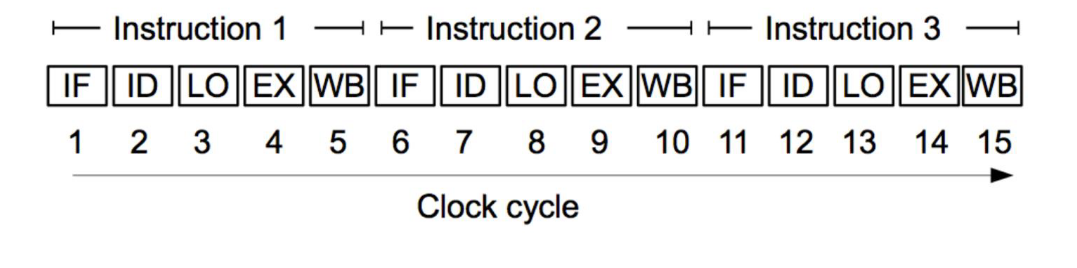
\includegraphics[scale=0.3]{immagini/no-pipeline}
\caption{Istruzioni senza pipeline}
\end{figure}
L'esecuzione in pipeline si basa sulla possibilità di sovrapporre le istruzioni, perché una istruzione non sta usando alcuni componenti della CPU che possono essere usate da altre
\begin{figure}[ht!]
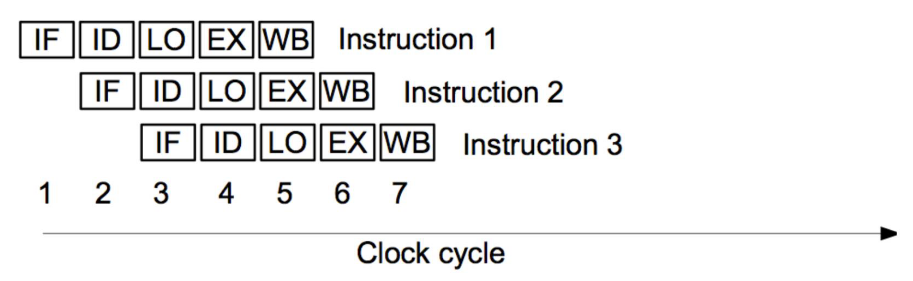
\includegraphics[scale=0.3]{immagini/pipeline}
\caption{Istruzioni con pipeline}
\end{figure}
Questo è l'ILP, e questo tipo di architettura è la base che, con altre tecniche, permettono di eseguire altro per affrontare problemi come il fatto che ogni operazione come la LO richieda più cicli di clock. Non sappiamo quanti cicli di clock richiede una istruzione, quindi il problema va affrontato. Inoltre, l'altro problema è legato ai \textbf{breaks:}se ho un'istruzione di salto e riesco a capire dove saltare solo quando l'istruzione è finalizzata, l'istruzione da mettere potrebbe essere differente da quella da immettere effettivamente e che si saprebbe solo alla fine. Questo è il problema della \textbf{control dependency}, altro problema è la \textbf{data dependecy}, dove il dato è richiesto da una istruzione in un momento in cui non è disponibile.\\ Analisi di cosa vuol dire usare pipeline: (vedi slides). Ovviamente, abbiamo uno speed up ideale, il problema è che non consideriamo i problemi sopra citati: non è detto che si riesce a committare una istruzione per ogni ciclo di clock, quindi possono essere richiesti molti più cicli di clock. Ampliando la pipeline, si amplia la \textbf{capacità di fare}, quindi inserire nel processore hw per fare operazioni che poi magari non vengono eseguite.
\subsection{Processori moderni}
Gli stage di pipeline non è molto elevato, quindi vediamo come è stato sfruttato per risolvere tutta la serie di problemi visti.\\ Abbiamo:
\begin{itemize}
\item software stall: inseriamo in un flusso di programma delle istruzioni di stallo fra due istruzioni. Se ho un salto e non so dove, metto degli stalli finché so se saltare o meno
\item software re-sequencing: fatto dai compilatori, quando si rendono conto che un blocco atomico di programma (ovvero un flusso eseguito tutto) si ri-organizza il blocco di istruzioni in modo che istruzioni che si dipendono siano più distanziate
\item per i salti, c'è la branch prediction: se non si sa quale è l'istruzione, si fa una previsione e si fa il fetch di quella zona di codice
\item out-of-order pipeline (OOO): la base di ciò che accade in una architettura moderna. Importantissimo per permettere alla CPU di essere efficace ed efficiente con generiche sequenza di istruzioni: se una istruzione deve aspettare dei dati, un'altra successiva può andare avanti ed anche completare \textbf{ma senza rendere visibili le cose nell'ISA}, o si viola il flusso di programma. Quindi, l'OOO non è basato su come le istruzioni toccano l'ISA, ma sul fatto che alcune istruzioni devono aspettare.
\end{itemize}
\subsection{Concetti base di x86}
Il processore x86 a 64 bit moderno ha più o meno lo stesso set di registri di un processore x86, la differenza è che sono un po' di più e sono più grandi.\\ I cambiamenti sono all'interno, ovvero come vengono eseguite le istruzioni: i486 è stato il primo ad adottare una architettura pipeline, riportata in seguito
\begin{figure}[ht!]
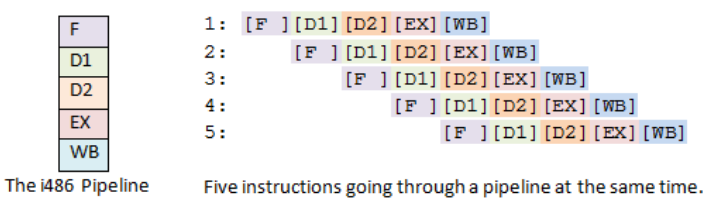
\includegraphics[scale=0.4]{immagini/pipeline-i486}
\caption{Pipeline di i468}
\end{figure}
L'architettura non è "piaciuta" molto, ad esempio per fare uno swap fra due registri questo richie 3 istruzioni, ma facendo diversi XOR ognuno dipende dal precedente, e questo rallentava tutta la pipeline.\\ Se ad esempio, abbiamo del codice C che accede ad un puntatore ed in un caso accede e poi incrementa il puntatore, oppure se accede dopo aver incrementato ha un effetto totalmente diverso. È possibile sperimentare lo stesso problema anche in linguaggi di più alto livello, ad esempio se si incrementa un puntatore:
\begin{itemize}
\item a = *++p
\item a = *p++
\end{itemize}
c'è una differenza in performance evidente fra i due statement.\\ C'è inoltre il problema di istruzioni che causano lo sqash della pipeline, ovvero viene cancellato tutto ciò che è contenuto nella pipeline. Tali istruzioni possono essere denotate come danno nel nostro programma, in quanto è possibile che vada rifatto il valore cancellato dalla pipe. Se consideriamo x86, una istruzione di questo tipo è \textsf{CPUID}, che prende l'ID numerico del processore su cui si sta lavorando. Questo è fondamentale quando si scrive del sw per il kernel, specialmente quando si sta scrivendo del sw che tocca delle strutture dati per lo specifico processore: bisogna conoscere quale è il processore su cui si lavora.\\ Tali istruzioni sono dette \textbf{serializing}, se però leggiamo il manuale dell'istruzione CPUID ci dice che è garantito che tutto ciò che viene fatto prima è stato completato prima che la prossima istruzione sia fetchata.
\subsection{Intel x86 superscalar pipeline}
Per superare il problema degli effetti del sw all'interno dell'esecuzione della pipeline richiede una  pipeline avanzata per capire cosa è possibile eseguire in parallelo etc: \textbf{superscalar pipeline}. Tale pipeline è fatta in modo che in ogni fase c'è più di un componente, ad esempio più componenti di esecuzione che possono essere identici e l'istruzione può andare in uno di essi. Se ad esempio l'istruzione richiede l'engine per più cicli di clock, non blocca successive istruzioni che magari poi richiedono lo stesso componente. C'è quindi parallelismo nella pipepline stessa, inoltre c'erano anche caratteristiche che faceva si che se c'era parallelismo e una istruzione stava passando avanti usando un'altra istanza del componente è che ciò che accade nella reale implementazione è che questa era basata su out-of-order: se qualche istruzione è ferma, le altre vanno avanti rispettando comunque il data flow model.\\ Tali aspetti erano nati molto prima, ad esempio nell'IBM 360/91 degli anni 60', si parlava però di architetture particolari.\\ Il tutto preveda che nella pipeline ci fossero altri componenti per gestire l'OOO.\\ Le basi del progetto erano:
\begin{itemize}
\item come mettere in commit le istruzioni in program order: fare uscire una istruzione dalla pipe indica che l'effetto dell'istruzione sulle risorse dell'ISA sono visibili, quindi è delicato capire quando mandare in commit
\item processare istruzioni indipendenti, sia sui dati che sulle risorse, il prima possibile
\end{itemize}
Il processore moderno ha una esecuzione differente da quello che accade in teoria nella pipeline: lo scenario in figura 1 è simulato, ma non è quello reale.\\ Vediamo come affrontare il problema che ogni istruzione possa durare un certo numero di cicli di clock
\subsubsection{Istruction span problem}
Ogni istruzione può durare un certo numero di clock, a seconda di cosa deve fare e per effetti diversi, ad esempio che occorre attendere componenti esterni alla CPU come la memoria. Il fetch dei dati può portare via diversi cicli di clock, e si è cercato di risolvere questo come problema centrale con le pipeline superscalari.\\ Con una OOO pipeline, può accadere la seguente cosa\\\\
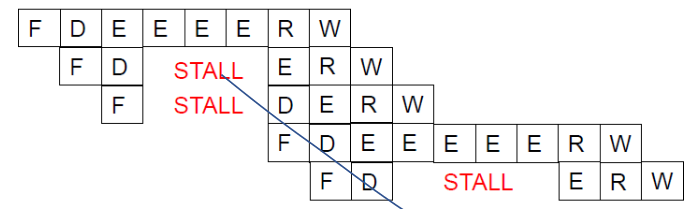
\includegraphics[scale=0.5]{immagini/ooo-pipeline-1}\\
può accadere che la seconda istruzione abbia uno stallo, magari perché non ha i dati. Come vediamo, in realtà l'istruzione ha bisogno di un solo ciclo di clock di esecuzione, ma ne usa di più perché non ha i dati disponibili. Anche la 3° istruzione è bloccata e lo stesso vale per l'ultima, perché deve usare lo stesso componente. Ricordiamo che il delay può avvenire perché il componente da usare non è pronto.\\ In OOO accade la seguente cosa:\\\\
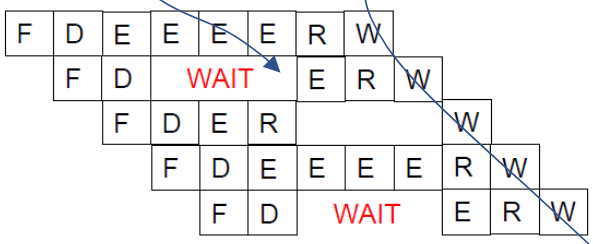
\includegraphics[scale=0.5]{immagini/ooo-pipeline-2}\\
può accadere che istruzione 1 e 2 usano due componenti identici nella pipeline, e 3 entra in esecuzione ed ha pronto il risultato molti cicli di clock prima di quando serve, quindi occorre mantenerla uncommitted e metterla in write back solo in maniera coordinata. Ad ogni ciclo di clock è possibile mandare in commitment il lavoro anticipato: se riusciamo a far entrare una istruzione ogni ciclo di clock, riusciamo a farne uscire una ogni ciclo di clock, avendo lo stesso throughput in ingesso ed in uscita rispetto alla pipeline tradizionale.
\subsection{Pipeline OOO speculativa}
Quando si parla di pipeline OOO, si parla anche di pipeline speculative: su un flusso di programma, se processiamo una istruzione successiva rispetto ad una che deve ancora essere processata, stiamo dicendo che c'è indipendenza fra le due, ma questo non è sempre vero. Quello che è in pipeline sta eseguendo in maniera speculativa, si fa fetch e poi magari le istruzioni non verranno eseguite perché si salta altrove. Inoltre, una istruzione in qualunque ciclo di clock può generare una trap: si potrebbe consultare il TLB (caching), ci rendiamo conto che qualcosa non va e quindi l'istruzione non può essere mandata in commit. Se c'è una trap mentre un program flow esegue, va passato il controllo ad un gestore lato sw, quindi tutte le istruzioni che venivano eseguite dopo erano eseguite in maniera speculativa.\\ Il \textbf{retire} è l'azione del committare una istruzione a rendere i cambiamenti "visibili" in termini di ISA, mentre l'\textbf{emissione} è l'azione di iniettare le istruzioni nella pipeline. Fra le due è possibile che ci siano altre istruzioni, ci sono poi anche le eccezioni che vanno gestite correttamente: se una istruzione entrata in pipeline genera una eccezione, ha senso eseguire un cambio di flusso per gestire l'evento particolare? No, in quanto l'istruzione è eseguita in modo speculativo. Finché non arriva alla fare di write back, questa può scomparire dal flusso, perché anche le istruzioni precedenti sono speculative e magari una istruzione precedente genera l'eccezione che rende l'eccezione di quella successiva inutile, perché l'istruzione non doveva proprio essere nel flusso di programma.\\ Quindi le eccezioni sono imprecise, non è detto che quando vengano generate queste esistano o meno, lo saranno solo se le istruzioni arriveranno al commit point.\\ Inoltre, l'eccezione viene generata considerando che in parallelo stiamo facendo altro in una OOO pipeline:
\begin{itemize}
\item una istruzione precedente è stata superata
\item una istruzione successiva ha superato
\end{itemize}
quindi quando viene generata la trap, lo stato effettivo del processore e quindi di tutti i componenti non esposti nell'ISA, globalmente può essere stato cambiato parzialmente da istruzioni che precedevano quella che ha generato la trap ma anche da istruzioni successive. Quindi, tutte queste istruzioni possono generare dei side effect, che possono essere sfruttati per attaccare le applicazioni ed i sistemi, prelevare dati a cui non si può accedere etc...\\ Di seguito, viene mostrato uno schema esemplificativo della pipeline OOO\\\\
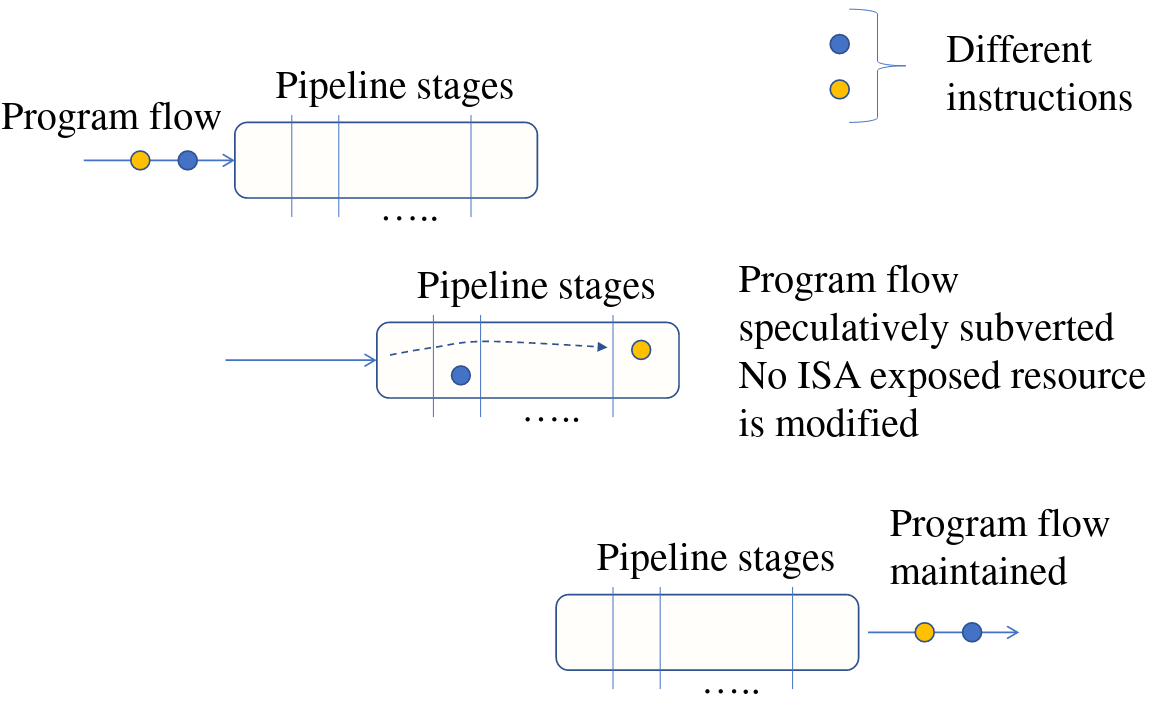
\includegraphics[scale=0.2]{immagini/pipeline-ooo}\\
può accadere che l'istruzione gialla arrivi prima a commit poi di quella blu, e questo permette di portare a termine lavoro utile anche quando altre istruzioni sono bloccate per i vari motivi detti prima.
\subsubsection{Eccezioni imprecise}
Su una architettura pipeline OOO (ma anche generale) in cui le istruzioni si superano l'un l'altra con un ILP molto elevato, consideriamo che una istruzione A è dopo una B nel program flow e B causa una eccezione. Quindi, B $\rightarrow$ A (B precede A), A entra in pipeline prima di B. Se B ha una eccezione, possono esserci tante altre istruzioni successive in pipeline e queste possono aver cambiato molto nello stato della CPU, tutte le relazioni di dipendenza possono essere portate avanti in maniera speculativa senza toccare i registri di CPU, ma toccando altri elementi. Può accadere che ci siano anche altre relazioni, ad esempio B genera dei valori che poi verranno usati da A e che A poi passi il risultato ad altre dopo etc... Si toccano componenti nella CPU in funzione del fatto che vengono anche passate informazioni in maniera speculativa e non a livello dell'ISA. Questo è stata la base dell'attacco meltdown, in cui è stata necessaria la patch di tutti i kernel esistenti: è possibile usare i processori OOO per leggere dati del kernel, è possibile leggere buffer cache e quindi leggere i file o i metadati per proteggere i dati (ad esempio dati di cifratura).
\subsection{Schema}
Quindi, se siamo in pipeline occorre stare attenti, altrimenti si scrive software di sistema non corretto. Può accadere che viene passato un output in maniera speculativa e che ci siano effetti su altri componenti della CPU. Vediamo dei dettagli su come è fatta una pipeline internamente.
\subsubsection{Algoritmo di Robert Tomaluso}
Le architetture moderne hanno delle varianti rispetto a questi algoritmi. Consideriamo come avviene il passaggio fra due istruzioni A e B per cui A$\rightarrow$B nel program flow, queste sono date perché:
\begin{itemize}
\item RAW (Read After Write): B legge dei dati prima che A li scriva, che porta ad uno stallo, dipendenza sui dati
\item WAW (Write After Write): B scrive dei dati prima A scriva lo stesso dato. Il dato espone un valore di stallo
\item WAR (Write After Read): B scrive un dato prima che A legga lo stesso dato, quindi il dato letto non è consistente.
\end{itemize}
Come risolviamo queste dipendenze sui dati: Tomasulo propone delle idee algoritmiche, per un processore OOO:
\begin{itemize}
\item RAW: per ciascuna lettura, bisogna tenere conto se il valore da leggere è già stato prodotto. Occorre quindi tenere traccia del fatto che il dato sia già stato prodotto, l'attesa del dato va quindi inserita nella OOO, quindi considerare il buffering dell'operazione
\item WAR e WAW: soluzione dei \textbf{renamed register}. Supponiamo di avere un registro R, per gestire WAw facciamo si che i due valori siano scritti ma sue due registri diversi. R non è un singolo registro, bensì è un multi-registro, dove ci sono varie versioni del dato. Qualsiasi istruzione deve scrivere un valore in un registro ed entra in pipeline va sul componente, preleva uno slot utilizzabile e scrive il valore in quello slot. Quindi, nel program flow può accadere che i valori possono essere scritti in tempi differenti sullo stesso registro, si risolve quindi WAW che si avrà in termini di commit del valore. Il valore non può sovrascrivere, perché viene scritto su uno slot, quando viene mandato in commit l'istruzione si avrà il valore effettivo associato al registro R, nel controller del registro c'è anche quale è la versione attuale del valore del registro.\\ Un solo valore alla volta è quello attivo, alcune versioni saranno del passato ed altre del futuro, nella storia dei commit che poi verrà realizzata.\\\\
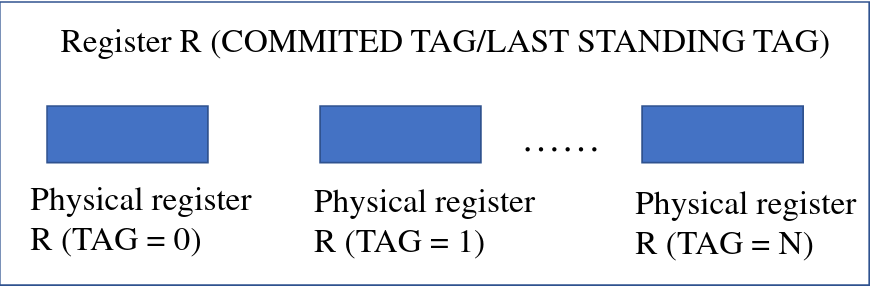
\includegraphics[scale=0.25]{immagini/multi-registri}\\
Quindi, quando mandiamo in pipeline una istruzione che deve leggere R, la marchiamo con il valore che quella deve leggere e finché il registro non è pronto l'istruzione rimane bloccata. Tutto questo è invisibili al programmatore in termini di risorsa ISA, ma visibile in termini del fatto che è possibile far si che il software faccia cambiare stato a tutti i registri in modo da creare problematiche.\\ In maniera indiretta è stato risolto anche WAR: per WAW è stato risolto il problema utilizzando i tag, ma anche per WAR finché il tag da leggere non è pronto, l'istruzione rimane ferma
\end{itemize}
\paragraph{Reservation stations}
Ogni istruzione ha un codice operativo, che va bufferizzato da qualche parte e poi va relazionato al componente che deve eseguire l'operazione. La reservation station è una zona del processore in cui viene registrata una operazione in input all'oggetto che può eseguire quella operazione, ad esempio somme etc... ai componenti corretti, ovvero che possono processarle. Non è detto che l'operazione venga processata immediatamente, perché può essere coinvolta in una dipendenza e dover attendere dei dati non ancora prodotti; questo viene detto dallo stato del renamed register. La reservation station riserva la possibilità di riservare il componente, finché l'istruzione non è pronta ad essere eseguita.
\paragraph{CDB e ROB}
Supponiamo di avere una reservation station in cui ci sia una operazione in coda: il flusso di informazioni fra le componenti deve essere supportato, che avviene usando il Common Data Bus, che permette di spostarle fra i vari componenti per permettere il corretto flusso di input fra le varie istruzioni.\\ C'è anche il Re Order Buffer: bisogna ricordarsi quale è l'ordine logico con cui andare a committare le operazioni, questo tiene conto dell'ordine. Viene gestito circolarmente e ogni slot viene liberato nel momento in cui viene committata l'operazione.
\\\\
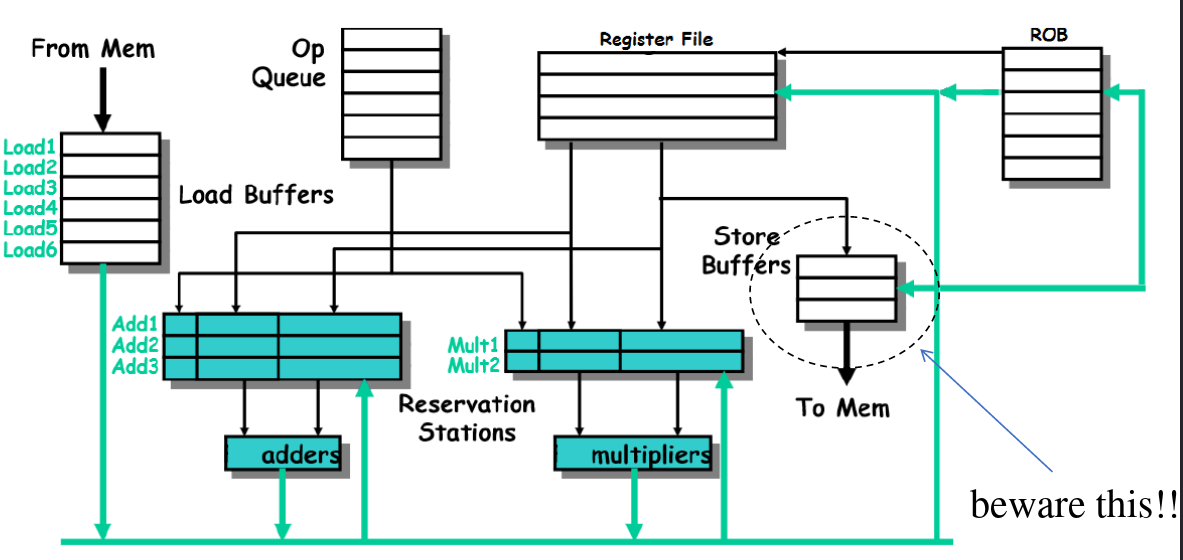
\includegraphics[scale=0.25]{immagini/arch-moderna}\\
Lo store buffer è un altro componente interessante: è fondamentale per interagire con la memoria. Mantiene in maniera temporanea il valore da scrivere per i dati verso la memoria. Lo SB viene toccato solo quando viene committata una istruzione, ed il valore viene scritto nello SB, non in memoria: in una architettura OOO quindi non si ottimizza solo il pipelining, ma anche la scrittura verso la memoria, perché se dovessimo scrivere in memoria a commit-time, la entry del ROB sarebbe occupata per vari cicli di clock e bloccherei diversi componenti senza poter andare avanti. Dallo SB i valori possono anche essere letti, e finché il valore non viene riportano in memoria è visto solo dal singolo program flow. Questo è il problema della sequential consistency, dove se qualcuno produce qualcosa questo non è visibile ad altri.\\\\ \textbf{esempio:} abbiamo 3 istruzioni che entrano in pipeline, con i rispettivi delay $\delta$ per essere processate.
\\\\
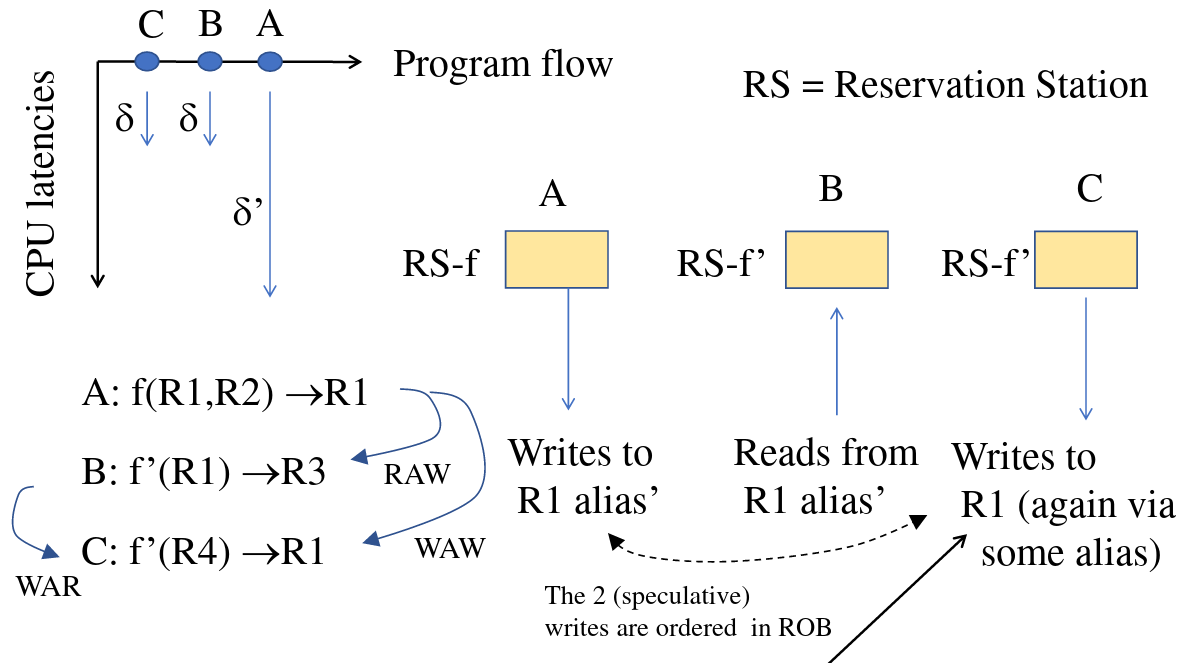
\includegraphics[scale=0.25]{immagini/ex-pipeline}\\
Questo è ciò che avviene realmente quando si esegue in pipeline di questo tipo istruzioni 
%slide dove fa vedere cosa accade
\subsubsection{Storia}
L'architettura basata sull'algoritmo di Tomasulo venivano mandate out of order solo determinate istruzioni, nei processori moderni l'OOO è visibile su tutto l'insieme delle istruzioni. Nell'evoluzione storica c'erano solo istruzioni in floating point, oggi si copre tutto il set di istruzioni
\subsection{Ancora sulla memoria}
Nel tempo, la memoria ha accelerato nella capacità di fornire informazioni, ma i processori hanno accelerato ancora di più nella richiesta delle chiamate a memoria. Quindi, guardando le 3 istruzioni precedenti ed i delay, ci sono anche i delay dovuti alla latenza per i miss in cache. Come vedremo, questo è stato il motivo della nascita delle architetture hyper-threading, ovvero la divergenza fra i due mondi.
\subsection{OOO nell'x86}
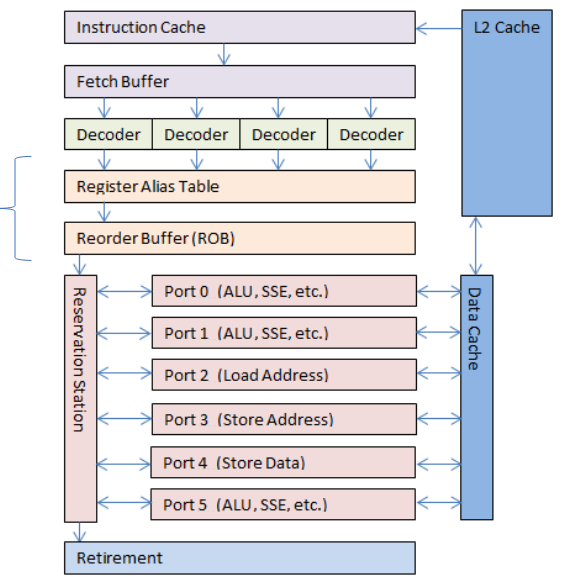
\includegraphics[scale=0.3]{immagini/x86-ooo}\\\\
A livello alto, nell'x86 abbiamo la Register Alias Table, il Reorder Buffer e tutta una serie di hardware replicato. Quando un oggetto entra nel Reorded Buffer, il firmware sceglie uno o l'altro componente replicato; ci sono poi le diverse relazioni che esistono fra i diversi componenti.\\ Questo fa capire che le istruzioni vengono caricate più alla volta, viene caricata una linea di cache che in 86 è da 64 byte, in cui si possono mettere diverse istruzioni, alcune andranno in commit ed altre no, però ci sono molte cose che si passano informazioni e fanno attività.
\subsubsection{Hyperthreading}
La necessità della nascita delle architetture hyper-threading è nata perché la struttura della CPU era talmente ottimizzata da rimanere senza fare nulla per troppo tempo, non riusciva più ad essere fillato in maniera efficiente quando i dati dovevano salire in memoria.\\ Le architetture ad hyper-thread prevedono che, siccome il "motore" è così rapido ed efficiente, si mandano due linee di input in parallelo, che sono due processori effettivi su un unico core: due program flow diversi su i due processori. Quando poi le istruzioni sono processate, si usa l'unico engine: il classico è avere 2-1 (es: 8 thread, 4 core). C'è una buona replicazione dei componenti, per evitare che se un flusso insista su un componente in particolare, non ci sia blocco.\\ Altro aspetto di sicurezza: c'è un interferenza fra i due thread in esecuzione che prevede che si vedano dati da uno all'altro, quindi bisogna "spegnere" uno dei due e sfruttare meno potenza effettiva.
\\\\
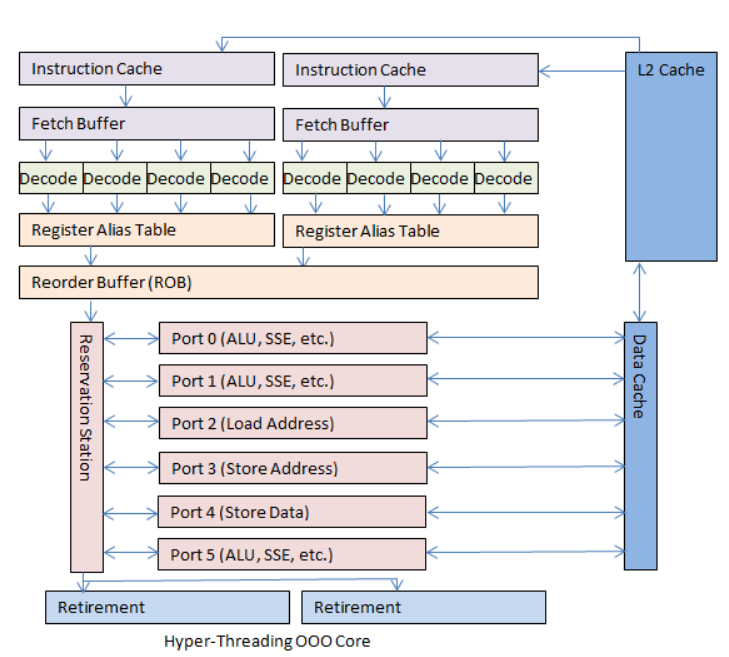
\includegraphics[scale=0.3]{immagini/hypert-ooo}\\
In questa architettura ci sono due hyper-thread ed una sola architettura per processare le istruzioni dei flussi e non c'è interferenza fra i due flussi, quindi quando l'istruzione scrive su un registro la risorsa è accessibile solo da quel flusso, ma la scrittura è tale per cui i componenti siano utilizzati per le istruzioni anche dell'altro flusso ma queste vengono usate in time sharing: gli oggetti non sono esposti nell'ISA, quindi questo non crea problemi a cosa è scritto nei programmi. In ogni caso, ci sono dei side effects sugli engine quando si esegue in hyper-threading, che sono problematici per la sicurezza.
\subsection{Gestione degli interrupt}
Ogni sistema moderno è interrupt-driven, quando c'è un interrupt bisogna eseguire una porzione di codice per rispondere agli interrupt.\\ Quando siamo sulla pipeline, avere un interrupt significa dire che siamo entrati con una serie di istruzioni sul thread corrente e l'interrupt vuole che si passi a prelevare istruzioni da un'altra zona di memoria, l'interrupt si accetta sempre quando una istruzione ha completato (per evitare di dover salvare lo stato dell'istruzione corrente). Per le altre istruzioni, che magari hanno già eseguito in maniera speculativa: o si salva lo stato della pipeline, oppure (più comodo) viene fatto lo squash della pipeline e si comincia a ri-fillare con le nuove istruzioni la pipeline. Questo ci fa capire che nei processori moderni l'interrupt costa: si butta del lavoro fatto e quasi finalizzato perché va squashato il contenuto nella pipeline, e quindi anche i valori scritti speculativamente negli alias dei registri.\\ Ci saranno delle policy per distribuire questa cosa su tutti i core presenti nell'architettura.
\subsection{Trap}
La trap è qualcosa di sincrono rispetto all'interrupt che è asincrono, capita perché il programma sta facendo qualcosa. Su una architettura pipeline, possono essere generate le seguenti trap in generali:
\begin{itemize}
\item Instruction Fetch \& Memory stages: l'istruzione può essere offending, quindi infinalizzabile. Page fault, ovvero l'indirizzo di memoria logico a cui accediamo non sappiamo a cosa corrisponda, accesso in memoria misaligned ovvero ci sono istruzioni che per lavorare correttamente hanno bisogno di indirizzi di memoria allineate ad una certa potenza di 2. Abbiamo poi memory and protection violation, ad esempio scrivere su una pagina read only: tale informazione viene data dalla page table e cachata nel TLB
\item Instruction decode stage: operazione illegale, un program counter ha detto lungo un program flow di prelevare l'istruzione ed eseguirla nel processore ma questa non è eseguibile dal processore. 
\item Execution stage: possono esserci problemi sull'esecuzione vera e propria, ad esempio divisione per 0
\item Write back: non ci sono eccezioni tipicamente
\end{itemize}
Noi, per una certa istruzione, possiamo subito accorgerci se l'istruzione è offending e quando la identifichiamo come offending nel momento in cui entra in pipeline e non l'ha ancora attraversata, cosa si fa? Si butta tutto il lavoro in pipeline? No, perché questa potrebbe aver superato altre istruzioni, quindi si rischierebbe di buttare cose che vanno finalizzate. Quindi come ci si comporta: si può far cambiare il flusso all'interno della pipeline, facendo attività differenti da eseguire nel momento in cui non fosse offending. Oppure è meglio marcarla con un bit ad 1, in modo da ricordarsi che è offending e quando arriva a commit point, la mando in abort e possono mandare in abort tutto il resto perché a quel punto tutto quello che era precedente è andato in commit.\\ Perché la scelta migliore è la 2, ed è stata applicata nell'architettura di processore: quando un'istruzione attraversa una pipeline, viene gestita da un micro-codice, ovvero un sotto-sistema di controllo che sa cosa fare per ogni tipo di istruzione. Per gestirla in maniera adeguata, dovrei avere un micro-codice apposito per gestire una istruzione offending in un certo punto, quindi questo comporterebbe una complessità maggiore nel micro-codice per la gestione delle istruzioni. Quindi si evitano transistor per introdurre ulteriore logica, quindi risparmio spazio per ampliare l'hardware per fare delle operazioni più utili.\\ Quindi si aggiunge un bit ad 1 per indicare che l'istruzione è offending, ma questo vuol dire che tutti gli altri passi dell'istruzione vengono portati avanti: tutto quello che si fa per quella istruzione è tale per cui tutto quello che l'istruzione sta facendo non era permesso. Ma se ho un memory access violation, l'istruzione nella pipeline può aver passato in un alias di registro le informazioni lette nel caso della violazione e può essere letta da una istruzione successiva, questo crea una serie di side effect: A accede a dei dati non permessi, li passa a B ed etc... i side effects generabili sono funzione dei dati acceduti e questo è un problema.\\ Questo è l'attacco meltdown
\subsection{Meltdown attack}
Supponiamo di avere a disposizione di un flusso di istruzioni in esecuzione un'area di memoria, dove abbiamo un array di 256 byte. Supponiamo di avere un byte in un altra locazione di memoria con un byte: possiamo scrivere un programma che usa questo byte come offset nell'array (essendo 256 possibili valori), accedendo quindi ad I[c]. Cosa è successo nell'architettura quando facciamo I[c]: abbiamo caricato c in memoria nel registro R ed usato R per accedere ad I. L'operazione di caricare c nel registro è in una architettura vera:
\begin{itemize}
\item può essere un'operazione speculativa, così come l'accesso in memoria usando il valore caricato di c
\item nell'architettura quello che accade e che un'istruzione ha chiesto di prendere c e metterlo in un registro. c è un RAM, per farlo fluire in un registro, c deve salire nell'architettura e passare per la cache. Quindi la lettura di c da usare come indice fa si che c passi comunque per la cache in una architettura moderna. Anche I[c] passa per la cache, se qualche istruzione vuole leggere questo byte deve passare anche lui per la cache.
\end{itemize}
Magari le due istruzioni sono offending, magari c è un valore inaccessibile al flusso di programma che è user-level e c è in zona kernel. L'istruzione va comunque avanti, con anche quelle successive, ma la cache ha cambiato stato. Quello che ha cambiato stato della cache è il fatto che uno dei caratteri è salito in cache, l'array potrebbe essere lecito perché magari è applicativo ed il che vuol dire che è stato creato un side effect per cui un suo byte è stato caricato in cache. Si può riaccedere all'array dopo aver eseguito questa istruzione? Si, eseguendo una funzione di gestione del segmentation fault e posso capire se dato un array di valori alcuni sono in cache ed altri no: basta leggerli e misurare il tempo di accesso al valore per distinguere fra cache hit ed cache miss. Quello in cache sarà esattamente in posizione c e quindi posso dedurre il valore di c e quindi di un byte kernel sapce che non avrei dovuto leggere.\\ Quindi meltdown funziona:
\begin{enumerate}
\item facendo cache flush, fattibile a livello user. Possiamo limitarlo anche solo all'array desiderato
\item leggiamo un byte di livello kernel
\item usiamo il byte per leggere una zona di memoria lecita, quindi in questo caso l'array detto prima
\item L'istruzione intermedia è offending, la zona successiva è phantom perché no esisterà in quanto non andrà in commit, ma possiamo vedere se ci sono stati dei side effects.
\end{enumerate} 
L'array della cache non è di caratteri, ma è di pagine: una cache line porta vari byte, un minimo di 64 su x86 ma anche il doppio o il triplo, quindi se leggo un byte l'architettura nel porta 128. Quindi il byte non va bene come unità di misura, non possiamo discriminare quale è il valore di c da inferire.\\ Le pagine sono di 4096 byte, e sono 256 pagine, usiamo C per accedere al 0-esimo byte della pagina, c identifica la pagina a cui ho acceduto. Se la pagina non è in cache assolutamente, non era in cache, se invece il byte 0 c'è ed è seguito da altri allora c identifica la pagina.\\ Nella demo ci sono due comandi cat del file /proc/nome\_file perché così facendo, chiedendo al kernel il dato e scrivendolo altrove, i cat portano in cache i dati del segreto che sto cercando di scoprire e quindi velocizzano nell'operazione di retrieve che si cerca di eseguire.
\paragraph{Side channel:}per portare a termine il meltdown, si usa un side channel. All'interno dell'esecuzione  possibile generare dei cambi di stato che non sono visibili nell'ISA, perché non esistono istruzioni per leggere il dato direttamente dalla cache, ma che possono essere osservati in altro modo. Alla base di tutti gli attacchi su macchine moderne ci sono i side channel
\subsection{Dettagli di x86 64 bit}
In x86 ci sono 16 registri general purpose, ma è retro compatibile con la versione a 32 bit in cui c'erano solo 8 registri a 32 bit.\\ I registri originali a 32 bit avevano determinati nomi ed è possibile utilizzarli ancora mediante il nome, per prendere i 32 bit meno significati del registro. Anche in un registro a 32 bit si possono gestire la metà del registro ed il singolo byte, lavorando a grana più fine, stesso vale per l'instruction pointer.\\ Ci sono poi altri registri per processare delle istruzioni particolari, che sono a 128 bit e poi dei registri per le istruzioni floating point.\\ Le istruzioni sono abbastanza e semplici similari:
\begin{itemize}
\item \textsf{mov\{b, w, l\}} (se byte, word o longword) \textsf{source dest}. Se non si specifica la size, la mov lavora a 64 byte
\item \textsf{push\{w, l\} source}
\item \textsf{pop\{w, l\} dest}
\end{itemize}
Per costruire un indirizzo per accedere alla memoria si può fare o con un indirizzo assoluto oppure specificando un offset all'interno dell'address space. In generale un indirizzo su x86 può essere targato con
\begin{itemize}
\item displacement, a questo possono essere sommati altri punti
\item base: può contenere un puntatore per accedere alla memoria
\item index + scale: altro offset che si può aggiungere ed è funzione di un pointer moltiplicato per un certo valore 
\end{itemize}
(slide che mostra come si muove x86).\\ Ci sono anche gli operatori logici ed istruzioni aritmetiche.
\subsubsection{Meltdown in assembly}
La sintassi intel prevede di usare prima il registro dest e poi src
%listato assembly
l'array è fatto di pagine di 4096 byte, quindi lo shift del contatore letto all'indirizzo kernel va fatto per indicizzare le diverse pagine, shiftando di 4096. Il valore trovato in rax può essere 0 se ho letto il valore 0, quindi salto su retry per rileggere lo stesso byte. Se accedo all'array, andrei nella prima pagina 0-esima e il valore 0 non è interessante perché è terminatore di stringa. Quindi aspetto che nella concorrenza qualcuno modifichi il valore letto. A quel punto, se non ho letto 0 carico in un altro registro quello che ho letto.\\ Speculativamente ha senso che tutto venga eseguito e che ci siano i side effects sulla cache, ma da un punto di vista reale non ha senso che venga eseguito.
\subsection{Contromisure per meltdown}
Per cercare di ovviare a queste problematiche di sicurezza dovute a meltdown:
\begin{itemize}
\item KASRL: Kernel Address Space Randomization, fa si che quando gira un applicazione, questa non sappia dove il kernel mantiene informazioni nella zona dell'address space. Se non sappiamo dove è mantenuta la chiave nell'address space del kernel bisogna andare verso attacchi bruteforce.\\ Il kernel, quando viene compilato, è pensato per avere le strutture dati e gli indirizzo a partire da una base nota. Con la randomizzazione, il kernel ad ogni statup si ricolloca a partire dalla zona nota, quindi è shiftata di un numero di posizioni che non conosciamo. Questo è possibile solo se gli accessi ai dati ed alle istruzioni in base al displacement avviene in base alla posizione relativa dall'istruction pointer.
\item KAISER, Kernel Isolation
\item Explicity cache flush ad ogni ritorno dal kernel mode: quindi se un flusso riprende il controllo dopo essere stato in kernel mode, si manda la cache in flushing. Ma possiamo avere una applicazione che, nell'asse temporale esegue come user, poi come kernel, poi di nuovo user etc... Se si fa questo la cache sta venendo buttata, quindi è come non averla in quanto viene sprecata in maniera sostanziale. Inoltre, ci sono anche attacchi che non passano per karnel.\\ La protezione può essere utile anche in un altro scenario: user eseguite in maniera malevola, quindi ci sono dei side effects che verranno osservati dopo. È possibile avere un percorso di questo tipo: eseguo, passo al kernel, il kernel esegue e mi rida il controllo. Se non valesse questa cosa, io saprei che le sys call che chiama il kernel durante quella esecuzione porta in cache dei dati che voglio attaccare. Quindi, potrei avere un attacco subito dopo la syscall.
\end{itemize}
La soluzione utilizzata ad oggi è KAISER, che sfrutta questa cosa: abbiamo analizzato le trap che possono capitare all'interno dell'attacco meltdown ovvero le memory protection violation. KAISER è tale per cui non è possibile generare quella trap per accedere a delle informazioni di zona kernel. In particolare, la page table per il programma ha le entry che afferiscono alla zona di address space user settate, mentre quelle che afferiscono alla zona kernel non sono settate e quindi generano trap di tipo page fault.\\ Ma è possibile avere una applicazione che quando esegue ha solo come pagine valide nella PT relative allo user space? No, è ideale: nell'address space, il kernel è visibile tramite la PT, il kernel non è reso tutto invisibile ma sono una zona. La zona visibile è l'unica usabile per entrare ed eseguire in modo kernel, una volta entrati si cambia la visibilità anche sul resto della zona. Quindi, in user space non si può accedere alle zone invisibili. L'implementazione attuale è la seguente: 
%immagine KAISER
due pt differenti, una per quando si lavora in maniera user ed una quando si lavora in kernel mode. Quando si chiama una sys call si passa ad una zona di address space in cui sono informazioni relative solo al codice kernel level, quindi non sensibile. In modo kernel, la zona di codice cambia la PT con una replicata in cui la zona è visibile, ma siamo già in modo kernel.\\ Il costo che viene pagato in termini del cambiamento della page table è che il TLB viene flushato. Nel TLB abbiamo una entry per una intera pagina, pagherò dei cache miss ma uno per pagina e non uno per ogni accesso come accade per la cache.\\ Inoltre, questa soluzione para da una serie di altri attacchi; la patch si può disattivare usando \textsf{pti=off} a livello del kernel usando GRUB. Su Linux è anche possibile mettere le patch on/off per la singola applicazione, se magari mi accorgo di un comportamento anomalo e non per tutte.
\end{document}
